\mode*
\part{Terminal}
\lecture{Terminal}{term}

\begin{itemize}
\item \citetitle[Sec.~5.3]{matthew2008beginning}
\item chap 62 of \citetitle{Kerrisk:2010:LPI:1869911}
\item \url{http://tldp.org/HOWTO/Text-Terminal-HOWTO-16.html}
\item \url{http://pubs.opengroup.org/onlinepubs/9699919799/}
\item[\$] \cmd{man infocmp}
\end{itemize}

History:
\begin{itemize}
\item In 1869, the \emph{stock ticker} was invented, which consisting of a typewriter, a
  long pair of wires, and a ticker tape printer. It can distribute stock prices over long
  distance in realtime.
\item Gradually, it evolved into the faster ASCII-based \emph{teletype}. Teletype were
  once connected across the world in a large network, called \emph{Telex}, which was used
  for transferring commercial telegrams.
\item Later came the computers. When the computers became powerful enough to be able to
  interact with users in realtime, the command line eventually replaced the old batch
  processing model. And teletypes were used as the I/O devices, because they were readily
  available on the market.
\item There was a plethora of teletype models around, all slightly different, so some kind
  of software compatibility layer was called for. 
\item In the Unix world, the approach was to let the OS kernel handle all the low-level
  details, such as word length, baud rate, flow control, parity, control codes for
  rudimentary line editing and so on. Fancy cursor movements, colour output and other
  advanced features made available in the late 1970s solid state \emph{video terminals}
  such as the VT-100, were left to the applications.
\item In present time, all the TTYs you're likely to see will be emulated video terminals
  --- software simulations of the real thing.
\item \emph{Why simulate these old things?} Because the command line interface is so handy
  that we cannot live without.
\end{itemize}

\begin{frame}{Terminal I/O Queue}
\begin{center}
  \mode<beamer>{ 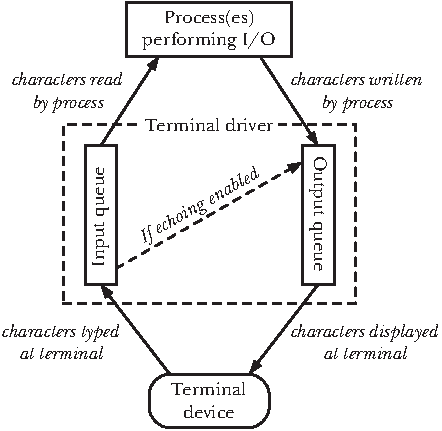
\includegraphics[width=.3\textwidth]{terminal-io-q} }%
  \mode<article>{ 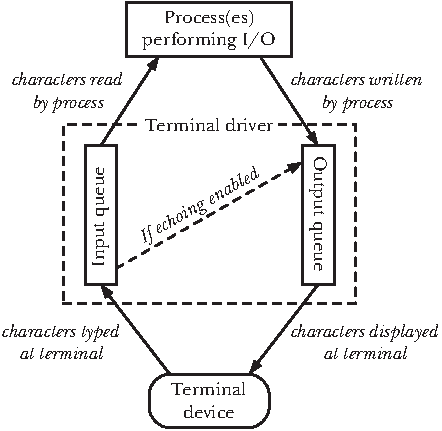
\includegraphics[width=.3\textwidth]{terminal-io-q} }
\end{center}
\end{frame}


\mode<all>
%%% Local Variables:
%%% mode: latex
%%% TeX-master: "lap-b"
%%% End:
